\documentclass{beamer}
\usepackage{graphicx}
\usepackage{amsmath}
\usepackage{kpfonts}
\usepackage{boxedminipage}
%\usepackage{bcprules}
\usetheme{CambridgeUS}
\usepackage{tikz}
%%%%%%%%%%%%%%%%Title Page%%%%%%%%%%%%%%%%%%%%%%%%%%%%%%%%%

\title[CS 251 Project]{CS 251 Project}
\subtitle[]{}
\author[F. last]{Data Pirates}
\institute[IITB]{
  Department of Computer Science and Engineering\\
  IIT Bombay.\\
  Powai, Mumbai - 400076\\[1ex]
  \texttt{180050025@cse.iitb.ac.in}
}
\date[\today]{\today}

%%%%%%%%%%%%%%%%%%%%%%%%%%%%%%%%%%%%%%%%%%%%%%%%%%%%%%%%%%%
\newtheorem{exercise}{Exercise}
\begin{document}
%--- the titlepage frame -------------------------%
%\begin{frame}[plain]
%  \titlepage 
%\end{frame}

%%%%%%%%%%%%%%%%%%%%%%%%%%%%%%%%%%%%%%%%%%%%%%%%%%%%%%%%%%%
\begin{frame}[fragile]{\bf  Implementation Details}
%\begin{enumerate}
\begin{block}{Database Design/Algorithm used}
\begin{enumerate}
\item We mainly use two tables in our data base
\item One table corresponds to the default user model provided by django and stores the attributes required to register and login.
\item Another comprizes Profile picture, Nick name and ID(foreign key) which is inner joined with the first table(where it's ID is the primary key).
\item Algo for password management: We use $auth\_password\_validators$ to validate the input password and flag appropriate error if the given requirements aren't met.
\end{enumerate}
\end{block}
%\end{enumerate}
\end{frame}

\begin{frame}[fragile]{\bf  Implementation Details}
\begin{block}{Workflow}
Most of the html files are extended from base.html
\end{block}
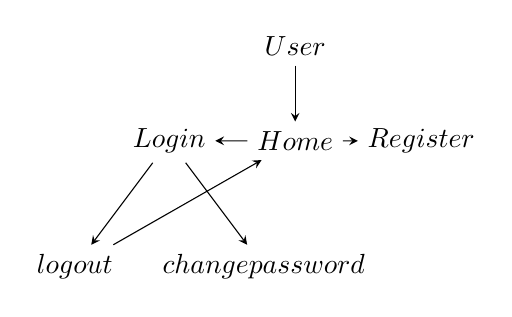
\begin{tikzpicture}[scale = 0.4]
\node (user) at (0, 0) {$User$};
\node (register) at (4,-3) {$Register$};
\node (login) at (-4,-3) {$Login$};
\node (home) at (0,-3) {$Home$};
\node (log out) at (-7,-7) {$log out$};
\node (change password) at (-1,-7) {$change password$};

\draw (user) edge[->,>=stealth] (home);
%\draw (home) edge[->,>=stealth,out=90,in=180,looseness=5] (home);
\draw (home) edge[->,>=stealth] (login);
\draw (home) edge[->,>=stealth] (register);
%\draw (register) edge[->,>=stealth,out=90,in=0,looseness=5] (register);
\draw (login) edge[->,>=stealth] (log out);
\draw (login) edge[->,>=stealth] (change password);
\draw (log out) edge[->,>=stealth] (home);
\end{tikzpicture}

\begin{block}{Reason for Choices Made}
We choose the provided user authentication template to keep it simple for the user and ourself. Later created a new model to accomodate user details in the database.  
\end{block}
\end{frame}
\begin{frame}[fragile]{\bf  Future Plan of Action}
\begin{block}{Future Timeline}
\begin{enumerate}
\item Planning on creating new tables for Friends, Groups ,and recent activity by creating new models for them.
\item All the new models contains $Transaction\_Id$ as the primary key and $User\_Id$ as the foreign key.
\begin{table}
\begin{tabular}{ c | c | c}
Friends & Groups & Activity tab \\
\hline \hline
User Id & User Id & User Id\\ 
Transaction Id & Transaction Id & Description\\
Friends Id & Friends Id & Transaction Id\\
Money & Money for friend & \\
Transaction time & Transaction time&\\
Description& Group name &\\
& Description &
\end{tabular}
\caption{Models for new database}
\end{table}
\end{enumerate}
\end{block}
\end{frame}

\begin{frame}[fragile]{\bf  Future Plan of Action}
\begin{block}{Reasoning for the additional feature selection}
Planning on taking up the second additional feature i.e notification management,when thers a settle up option.
For this, we are planning on creating another tab in the frontend and a model in the backend for notifications. 
\end{block}
\begin{block}{Detailed plan}
\begin{enumerate}
\item Existing tables are to be extensively used.
\item For example, date ranges can be accessed from Friends and Groups tab and we can list out the transactions pertaining to that range.
\item to get the bar graphs, pie chart, time series plot, Matplotlib in python can be used. 
\end{enumerate}
\end{block}
\end{frame}
\end{document}
